\chapter{Primo sguardo all'analisi algoritmica}

\section{Definizione e proprietà degli algoritmi}

Prima d'iniziare ad analizzare un algoritmo dobbiamo prima capire cos'è un algoritmo.

\dfn{Algoritmo}{
    Un \textbf{algoritmo} è una procedura ben definita che prende un certo valore, o un insieme di valori, come \textbf{input} e genera un valore, o un insieme di valori, come \textbf{output}.
}

Quindi un algoritmo lo possiamo interpretare come \textit{una sequenza finita di passi} che,
se eseguiti da un \textbf{esecutore}, portano alla soluzione di un \textbf{problema computazionale} ben definito.

In generale un algoritmo gode delle seguenti proprietà:
\begin{itemize}
   \item \textbf{Non ambiguità:} tutti i passi che definiscono l'algoritmo devono essere non ambigui e chiaramente comprensibili dall'esecutore;
	\item \textbf{Generalità:} la sequenza di passi da eseguire dipende esclusivamente dal problema generale da risolvere, non dai dati che ne definiscono un'istanza specifica;
	\item \textbf{Correttezza:} un algoritmo è \textbf{corretto} se produce il risultato corretto a fronte di qualsiasi istanza del problema ricevuta in ingresso. Può essere stabilita, ad esempio, tramite:
	\begin{itemize}
		\item dimostrazione formale (matematica);
		\item ispezione informale;
	\end{itemize}
	\item \textbf{Efficienza:} misura delle risorse computazionali che esso impiega per risolvere un problema. Alcuni esempi sono:
	\begin{itemize}
		\item tempo di esecuzione;
		\item memoria impiegata;
		\item altre risorse: banda di comunicazione.
	\end{itemize}
\end{itemize}

\subsection{Il tempo di esecuzione di un algoritmo}

Spesso, quando si analizzano le proprietà di un algoritmo si parla di \textbf{complessità computazionale}. Questa può essere definita come segue:

\dfn{Complessità computazionale}{
    La \textbf{complessità computazionale} è il costo, in termini di tempo e memoria, necessari per eseguire un algoritmo, quindi per risolvere un problema.
}

Per determinare la complessità computazionale di un algoritmo bisognerà quindi definire al meglio il concetto di \textit{tempo di esecuzione}.

\dfn{Tempo di esecuzione}{
Il \textbf{tempo di esecuzione} di un programma per un particolare input è il numero di operazioni primitive che vengono eseguite o ``passi''.
}

Il tempo di esecuzione può dipendere da vari fattori:
\begin{itemize}
	\item Hardware su cui viene eseguito;
	\item Compilatore/Interprete utilizzato;
	\item Tipo e dimensione dell'input;
	\item Altri fattori: casualità
\end{itemize}

Una misura del costo computazionale soddisfacente deve:
\begin{enumerate}
    \item Basarsi su un \textbf{modello computazionale} in modo tale da poter definire il concetto di \textbf{passo algoritmico} nel modo più indipendente possibile dal tipo di esecutore;
    \item Svincolarsi dalla configurazione dei dati in ingresso, ad esempio basandosi sulle configurazioni più sfavorevoli (caso peggiore), così da garantire che le prestazioni nei casi reali saranno al più costose quanto il caso analizzato;
    \item Essere una funzione della dimensione dell'input;
    \item Essere asintotica, cioè fornire un'idea dell'andamento del costo all'aumentare della dimensione dell'input\footnote{Senza essere troppo precisi nell'analisi della grandezza di tale input. Nel nostro caso di studio infatti non stiamo considerando la macchina effettiva che esegue il calcolo.}.
\end{enumerate}

Una misura del costo computazione di un algoritmo deve quindi fornire una descrizione del costo asintotico nel caso peggiore, ovvero l'insieme degli input per i quali l'algoritmo richiede il massimo tempo di esecuzione.


\subsubsection{La macchina di Turing}\label{sez:Turing}
Alla base di un modello computazionale sta l'idea che ogni istruzione atomica abbia un \textbf{costo unitario}. Un noto modello computazionale è il modello della \textbf{macchina di Turing (MdT)}. Si tratta di una macchina astratta che manipola i dati contenuti su un nastro di lunghezza potenzialmente infinita, secondo un insieme prefissato di regole ben definite. Questo modello è largamente utilizzato nella teoria della calcolabilità e nello studio della complessità degli algoritmi, in quanto è di notevole aiuto agli studiosi nel comprendere i limiti del calcolo meccanico; la sua importanza è tale che oggi, per definire in modo formalmente preciso la nozione di algoritmo, si tende a ricondurlo alle elaborazioni effettuabili con macchine di Turing.

Una MdT, come mostrato in Figura \ref{fig:mdt}, è composta da:
\begin{itemize}
    \item Un \textbf{nastro di lunghezza infinita} costituito da celle le quali possono contenere una quantità d'informazione finita.
    \item Una \textbf{testina}, un \textbf{processore}, un \textbf{programma}
\end{itemize}

Le operazioni che può compiere in una \textbf{singola unità di tempo} sono:
\begin{itemize}
    \item Leggere o scrivere nella cella puntata attualmente dalla testina;
    \item Muoversi di una cella a destra, a sinistra oppure restare ferma.
\end{itemize}

\begin{center}
    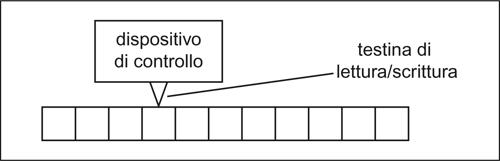
\includegraphics[scale = 0.4, origin = c]{res/Macchina_di_Turing.jpg}
    \captionof{figure}{Macchina di Turing}\label{fig:mdt}
\end{center}

\section{Algoritmo conta coppie}
Proviamo a studiare un algoritmo che fa quanto segue:
\begin{itemize}
    \item \textbf{Input:}  $n\in\mathbb{N}^*$, dove per $\mathbb{N}^*$ si intende $\mathbb{N}\setminus\{0\}$.
    \item \textbf{Output:} numero di coppie $(i,j)$ con $1\leq i\leq j\leq n$
\end{itemize}
Ad esempio, per $n=4$ abbiamo $10$ casi: $(1,1),(1,2),(1,3),(1,4),(2,2),(2,3),(2,4),(3,3),(4,4)$.

\subsection{Un metodo di risoluzione na\"if}
Il primo step per risolvere un problema difficile è quello di \textbf{decomporlo in problemi più semplici} seguendo l'approccio \emph{divide et impera}. L'idea quindi sarebbe quella di generare tutte le coppie e successivamente contare quelle che soddisfano la condizione posta. Si ottiene così:


\begin{lstlisting}[label=lst:Conta1, language=asd, caption={Conta1(n)}]
RIS = 0
for i = 1 to n do
    for j = 1 to n do
        if i <= j then
            RIS = RIS + 1
return RIS
\end{lstlisting}

Bisogna adesso porsi il problema di come associare un tempo di esecuzione all'Algoritmo \ref{lst:Conta1}. Nel farlo assumiamo che il valore dell'input sia \textbf{misura della complessità dell'algoritmo}\footnote{In generale non sarà così ma assumiamo che nel nostro modello computazionale i dati vengano rappresentati attraverso un sistema unario.}. Analizziamo la complessità di \textit{ogni linea} contandone le operazioni elementari e valutando il numero di volte in cui queste vengono eseguite:
\begin{enumerate}
  \item L'istruzione contiene una singola operazione elementare che viene eseguita a tempo costante.
  \item Il ciclo \texttt{for} viene eseguito $n+1$ volte. Infatti, oltre alle $n$ iterazioni date dall'estremo superiore, viene effettuata un'iterata in più per il controllo che permette all'esecutore di uscire dal ciclo una volta che la condizione risulta falsa. Il contributo della riga sarà quindi:
	\begin{displaymath}
		2 \cdot \sum_{i=1}^{n+1}=2 \cdot (n+1)
	\end{displaymath}
  \item Questo ciclo si trova annidato al primo ciclo \texttt{for}. Quindi ciascuna delle sue $n+1$ iterazioni sarà ripetuta $n$ volte. In totale:
	\begin{displaymath}
		2 \cdot \sum_{i=1}^{n} (\sum_{j=1}^{n+1} 1 )= 2 \cdot \sum_{i=1}^{n}(n+1)=2 \cdot n \cdot (n+1)
	\end{displaymath}
  \item L'istruzione \texttt{if} si trova all'interno dei due cicli for, sarà quindi ripetuta:
	\begin{displaymath}
		3 \cdot \sum_{i=1}^{n}(\sum_{j=1}^{n} 1) = 3 \cdot n^{2}
	\end{displaymath}
	volte.
  \item È impossibile determinare a priori il numero di volte in cui l'istruzione all'interno dell'istruzione \texttt{if}, essendo questo dipendente dal soddisfacimento o meno della condizione imposta alla coppia $(i,j)$. Nel caso in questione possiamo osservare che, se $i=1$, il corpo dell'\texttt{if} viene eseguito $n$ volte; con $i=2$ viene eseguito $n-1$ volte, $\ldots$ con $i=k$ viene eseguito $n-(k-1)$, dove $k$ è il valore corrente di $i$. In generale:
  \begin{displaymath}
  \sum_{i=1}^{n} (n-i+1)
  \end{displaymath}
\end{enumerate}

Per calcolare l'ultima sommatoria basta spezzarla in tre sommatorie:
\begin{equation}
    \sum_{i=1}^{n} (n-i+1) = \sum_{i=1}^{n} n - \sum_{i=1}^{n} i + \sum_{i=1}^{n} 1 = n^2 - \frac{n(n+1)}{2} + n = n(n+1) - \frac{n(n+1)}{2} = \frac{n(n+1)}{2}
\end{equation}

Ora per calcolare il tempo di esecuzione, basta sommare:
\begin{eqnarray*}
    T_1(n) &=& 1+ 2\cdot(n+1) + 2\cdot(n^{2}+n)+3n^{2} + \frac{n(n+1)}{2} \\
    &=& 1 + 2n + 2 + 2n^2 + 2n + 3n^2 + \frac{n^2}{2} + \frac{n}{2} \\
    &=& \frac{11}{2}n^2 + \frac{9}{2}n + 4
\end{eqnarray*}

Il nostro algoritmo ha tempo \textbf{quadratico}. È facile convincersi del fatto che l'algoritmo\ref{lst:Conta1} è molto laborioso in quanto deve generare ben $n^{2}$ coppie quando potrebbe sicuramente generarne di meno.

\subsection{Migliorare l'algoritmo tramite l'analisi}
L'analisi del tempo di esecuzione dell'Algoritmo \ref{lst:Conta1} ci ha permesso di prevedere all'$i$-esima iterazione del \texttt{for} a linea 2 quante volte veniva eseguita il corpo dell'\texttt{if}. Proviamo a usare questa conoscenza a nostro vantaggio per migliorare l'algoritmo.

Ciò che si era notato era che, fissato $i$, non c'è bisogno di effettuare alcun controllo in quanto il numero di coppie $(i,j)$ che soddisfano alla nostra condizione è pari a $\displaystyle\sum_{i=1}^{n} (n-i+1)$, ovvero:
\begin{equation}
    \frac{n(n+1)}{2}
\end{equation}

A questo punto proviamo a scrivere il nuovo codice utilizzando questo concetto.

\begin{lstlisting}[label = lst:Conta2, language=asd, caption={Conta2(n)}]
RIS = 0
for i = 1 to n do
    RIS = RIS + (n-i+1)
return RIS
\end{lstlisting}

Analizzando nuovamente, istruzione per istruzione, il costo computazionale dell'algoritmo si evince che $T_2(n) = 9n+4$. Infatti:
\begin{enumerate}
  \item Tempo costante;
  \item $2\ \displaystyle\sum_{i = 1}^{n+1} 1 = 2n+2$;
  \item $(3+3+1) n = 7n$;
  \item Tempo costante.
\end{enumerate}

Il nostro algoritmo è migliorato in quanto adesso il tempo di esecuzione è lineare. Da quadratico a lineare è un grande miglioramento, ma possiamo fare di meglio. Infatti, adesso l'algoritmo non fa nient'altro che calcolare $\displaystyle\sum_{i=1}^{n} i$ di cui, come abbiamo già osservato, esiste una diretta correlazione con la somma dei primi $n$ numeri. I due problemi sono infatti isomorfi. Dunque abbiamo:

\begin{lstlisting}[label = lst:Conta3, language=asd, caption={Conta3(n)}]
RIS = (n(n+1))/2
return RIS
\end{lstlisting}

\textbf{Tempo di esecuzione per ogni istruzione:}
\begin{enumerate}
  \item 2 + 3 = 5
  \item 1
\end{enumerate}

Dall'analisi si evince che $T_3(n) = costante$.


\section{Somma della massima sottosequenza}\label{sottosequenzecontigue}
Proviamo a studiare un algoritmo che fa quanto segue:
\begin{itemize}
    \item \textbf{Input:}  $n\in\mathbb{N}^*, A$. Dova A è un array di dimensione N
    \item \textbf{Output:} La somma della massima sotto-sequenza di A
\end{itemize}

\begin{example}
		Sia $n=7$, e consideriamo l'array: \{1, -3, 8, 2, -10, 1, 7\}. In questo caso, la massima sottosequenza ha somma 10, infatti: $MaxSum = 8+2$.
\end{example}

\subsection{Introduzione e prima risoluzione del problema}
Una prima idea, potrebbe essere quella di applicare un algoritmo \textit{\textbf{brute force}}.
Quindi dobbiamo applicare i seguenti passi:
\begin{enumerate}
    \item Generare tutte le possibili sotto-sequenze.
    \item Calcolarne la somma.
    \item Aggiornare il max.
\end{enumerate}

Per generare tutte le possibili sotto-sequenze possiamo scegliere di rappresentarla con una coppia $(i, j)$, dove $i$ è l'indice del primo elemento, e $j$ quello dell'ultimo, tale che $i\leq j$.


\begin{lstlisting}[label = MaxSum1, language=asd, caption={MaxSum1(A,n)}]
MAX = 0
    for i=1 to n do
        for j=i to n do
            SUM = 0
            for k=i to j do
                SUM = SUM + A[k]
            if SUM > MAX then
                MAX = SUM
return MAX
\end{lstlisting}

Effettuando un'analisi non approfondita ci rendiamo conto dai tre cicli \texttt{for} innestati che l'algoritmo in questione ha un costo cubico $(T_1 = O(n^3))$ rispetto all'input. Notare che nell'algoritmo \ref{MaxSum1} vengono effettuate diverse volte le stesse operazioni, questo perché andiamo a calcolare ogni volta da capo la somma, infatti:
\begin{equation}
    \sum_{k=i}^{j+1} A[k] = \sum_{k=i}^{j} A[k] + A[k+1]
\end{equation}

Dove $\displaystyle\sum_{k=i}^{j} A[k]$ è l'operazione ripetuta più volte. Per migliorare questo aspetto, possiamo conservare la somma e aggiungere solo il successivo per ogni sequenza. Vediamo come evolve il codice dopo questa modifica.

\begin{lstlisting}[label = MaxSum2, language=asd, caption={MaxSum2(A,n)}]
MAX = 0
for i=1 to n do
    SUM = 0
    for j=i to n do
        SUM = SUM + A[j]
        if SUM > MAX then
            MAX = SUM
return MAX
\end{lstlisting}

Questa modifica ci consente di ridurre il costo del nostro algoritmo da cubico a quadratico. $T_2 = (O(n^2))$.

\subsection{Algoritmo \textsc{MaxSum} lineare}

Prima di procedere a scrivere l'algoritmo, fermiamoci a ragionare sul come possiamo ``scartare'' parti di array, in modo da non doverlo controllare tutto per cercare la massima sotto-sequenza. Per semplicità consideriamo di avere solo tre valori: $a$, $b$, $c$. Di questi, ipotizziamo siano vere:
\begin{enumerate}
    \item $a<b$;
    \item $b<c$.
\end{enumerate}
Quindi per transitività sappiamo che $a<c$. Potrà sembrare una banalità, ma così facendo risparmiamo un confronto, ed è proprio la chiave per ottimizzare l'algoritmo. Ipotizziamo sia vero quanto segue:

\begin{equation}
    \sum_{z=i}^{j} A[z] \geq 0 \text{ , con } i \leq j \leq r-1
\end{equation}

Si hanno allora due possibili casi:

\begin{enumerate}
    \item $\displaystyle\sum_{z=i}^{r} A[z] \geq 0$, allora:
    \begin{displaymath}
        \sum_{z=i}^{k} A[z] = \sum_{z=i}^{j} A[z] + \displaystyle\sum_{z=j+1}^{k} A[z] \geq \displaystyle\sum_{z=j+1}^{k} A[z]
    \end{displaymath}
    Se $a$ un numero sommo una quantità positiva, ottengo un numero più grande, banalmente. Di conseguenza
    è inutile calcolare le sottosequenze interne ad $i$ ed $r$.

    \item $\displaystyle \sum_{z=i}^{r} A[z] < 0$, allora:

    \begin{displaymath}
        \sum_{z=j}^{k} A[z] = \sum_{z=i}^{r} A[z] + \sum_{z=r+1}^{k} A[z] < \sum_{z=r+1}^{k} A[z]
    \end{displaymath}

    Sappiamo che la prima sommatoria è negativa semplicemente perché per ipotesi $\displaystyle\sum_{z=i}^{j-1} A[z] + \sum_{z=j}^{r} A[z] < 0$.

    Ricapitolando, $\displaystyle\sum_{z=j}^{k} A[z] \leq \sum_{z=r+1}^{k} A[z]$, cioè è inutile calcolare ogni sottosequenza che inizia tra $i$ ed $r$ e termina oltre $r$.
\end{enumerate}

Facendo questa analisi siamo riusciti a eliminare un gran numero di calcoli e confronti superflui. Andiamo a vedere come evolve l'algoritmo.


\begin{lstlisting}[label = lst:MaxSum3, language=asd, caption={MaxSum3(A, n)}]
MAX = 0
SUM = 0
for i=1 to n do
    SUM = SUM + A[i]
    if SUM < 0 then
        SUM = 0
    else
        MAX = MAX(SUM, MAX)
return MAX
\end{lstlisting}

Andando a fare un'analisi del codice vediamo che abbiamo un solo \texttt{for} che va da $1$ a $n$, ovvero, andiamo a eseguire tante istruzioni quanto $n$.

In conclusione, andando a eliminare confronti e calcoli superflui, siamo riusciti nell'intento di rendere il nostro algoritmo lineare. $T_3 = O(n)$.
